\documentclass[%
reprint,
%superscriptaddress,
%groupedaddress,
%unsortedaddress,
%runinaddress,
%frontmatterverbose, 
%preprint,
%preprintnumbers,
%nofootinbib,
%nobibnotes,
%bibnotes,
 amsmath,amssymb,
 aps,
%pra,
%prb,
%rmp,
%prstab,
%prstper,
%floatfix,
]{revtex4-2}

\usepackage{subfiles}
\usepackage{graphicx}% Include figure files
\usepackage{dcolumn}% Align table columns on decimal point
\usepackage{bm}% bold math
\usepackage{float}
\usepackage{mathtools}
%\usepackage{hyperref}% add hypertext capabilities
%\usepackage[mathlines]{lineno}% Enable numbering of text and display math
%\linenumbers\relax % Commence numbering lines

%\usepackage[showframe,%Uncomment any one of the following lines to test 
%%scale=0.7, marginratio={1:1, 2:3}, ignoreall,% default settings
%%text={7in,10in},centering,
%%margin=1.5in,
%%total={6.5in,8.75in}, top=1.2in, left=0.9in, includefoot,
%%height=10in,a5paper,hmargin={3cm,0.8in},
%]{geometry}

\newcommand{\Hp}{\mathcal{H}}

\begin{document}

\section{The CMB and matter power-spectra}
\label{sec:4}
Now that we have solved the background cosmology, retrieved relevant data from the era of recombination and solved the perturbations on the background cosmology we are finally in a position to compute the CMB power spectrum. Since we have already calculated $\Theta_\ell(k,x)$, all we need to do to find the coefficients is to read in this data at time $x=0$. One problem we have is that since we only computed to $\ell_\text{max}=7$ in the prior section, and we would like to probe smaller regions than this, e.g. $\ell_{\text{max}}=2000$. This would be incredibly slow with our code so we need to consider a new technique to compute this. To do this we use the so-called line-of-sight integration technique to be introduced in the theory section.

\subsection{Theory}

\subsubsection{Line-of-sight integration}
The idea behind line-of-sight (LOS) integration is that instead of performing a multipole expansion on equation (\ref{eq:LOS_thingy}) we begin by integrating the equation for $\dot\Theta$ and perform the multipole expansion afterwards. Doing this one arrives at
\begin{align*}
	\Theta(k,\mu,\eta_0)=\!-\!\int_0^{\eta_0}&\left[\dot\Phi\!+\!ik\mu\Psi\!+\!\dot\tau\left(\Theta_0\!+\!i\mu v_{\text{B}}\!-\!\frac{P_2}{2}\Theta_2\right)\right]\\
	&\times e^{ik\mu(\eta-\eta_0)-\tau}d\eta
\end{align*}
where $\eta_0\equiv\eta(x=0)$. Here we can switch out any factors of $\mu$ with a derivative w.r.t. $\eta$ and the necessary coefficients. Expanding in multipoles, integrating over $\mu$ and using the definition of Bessel functions $j_\ell$:
\[\frac{i^\ell}{2}\int_{-1}^1d\mu\,P_\ell(\mu)e^{ik\mu(\eta-\eta_0)}=j_\ell[k(\eta_0-\eta)], \]
we arrive at
\begin{align}
	\Theta_\ell(k,\eta_0)=\int_0^{\eta_0}d\eta\,S(k,\eta)j_\ell[k(\eta_0-\eta)],
	\label{eq:LOS}
\end{align}
where the source function $S(k,\eta)$ is defined as
\begin{align*}
	S(k,\eta)&=\tilde{g}\left[\Theta_0+\Psi+\frac{1}{4}\Theta_2\right]+e^{-\tau}\left[\dot\Psi-\dot\Phi\right]\\
	&-\frac{1}{k}\frac{d}{d\eta}(\tilde{g}v_\text{B})+\frac{3}{4k^2}\frac{d^2}{d\eta^2}(\tilde{g}\Theta_2).
\end{align*}
Rewriting (\ref{eq:LOS}) in terms of $x$ we then have
\begin{align}
	\Theta_\ell(k,x=0)=\int_{-\infty}^0dx\,\tilde{S}(k,x)j_\ell[k(\eta_0-\eta)],
	\label{eq:LOSx}
\end{align}
where the source function in terms of $x$ and in SI units now reads
\begin{align}
	\tilde{S}(k,x)&=\tilde{g}\left[\Theta_0+\Psi+\frac{1}{4}\Theta_2\right]+e^{-\tau}[\Psi'-\Phi']\nonumber\\
	&-\frac{1}{ck}\frac{d}{dx}(\Hp\tilde{g}v_\text{B})+\frac{3}{(2ck)^2}\frac{d}{dx}\left[\Hp\frac{d}{dx}(\Hp\tilde{g}\Theta_2)\right],\label{eq:source_function}
\end{align}
which is what we will be using. For reference, the final term of the source function expanded yields
\begin{align*}
	\frac{d}{dx}\left[\Hp\frac{d}{dx}(\Hp\tilde{g}\Theta_2)\right]=\tilde{g}''\Hp^2\Theta_2+\tilde{g}'(3\Hp\Hp'\Theta_2+2\Hp^2\Theta_2')\\
	+\,\tilde{g}(\Hp'^2\Theta_2+\Hp\Hp''\Theta_2+3\Hp\Hp'\Theta_2'+\Hp^2\Theta_2'').
\end{align*}
Now we can easily see that the only quantities which we need to calculate arbitrarily high $\ell$'s are ones which we have already calculated in the previous sections together with the corresponding Bessel functions $j_\ell$. 


\subsubsection{CMB power spectrum}
With a nice computational trick in hand what remains is to translate the $\Theta_\ell$ into more convenient observables which we can measure. In order to do this from our various computed quantities we first recall the definition of the spherical harmonics transform of the CMB temperature
\[T(\hat{n})=\sum_{\ell=0}^\infty\sum_{m=-\ell}^\ell a_{\ell m}Y_{\ell m}(\hat n)\]
where $\hat{n}$ is the direction in the sky, $Y_{\ell m}$ are the spherical harmonics and $a_{\ell m}$ are their coefficients. Since inflation predicts initial perturbations to be Gaussian random fields, the spherical harmonic coefficients $a_{\ell m}$ must also satisfy this. Thus we define the variance of these coefficients $C_\ell$ to be
\[C_\ell\delta_{\ell\ell'}\delta_{mm'}\equiv\langle a_{\ell m}^*a_{\ell' m'}^{\phantom{*}}\rangle,\]
where $C_\ell$ is the \textbf{angular power spectrum}. Note here that since the Universe is approximately isotropic we must have the same power spectrum in the various directions; as such we average over $m$ and drop the subscript. For each fixed $\ell$, every $a_{\ell m}$ contain the same variance and there are $2\ell+1$ possible values for $m$. Thus to estimate $C_\ell$ from a given measurement we can estimate the power spectrum as
\[\hat C_\ell=\frac{1}{2\ell+1}\sum_{m=-\ell}^\ell |a_{\ell m}|^2.\]
Up until now our theory has been formulated in terms of an ensemble average; however we only have one manifestation of this ensemble to perform measurements on, namely our universe. Due to this, simple statistics then tell us that we will have a large uncertainty on the angular power spectrum for low $\ell$'s. This can be easily understood by just considering that for e.g. $\ell=2$ we only have 5 patches in the sky to work with, thus we may only have 5 data points which will lead to a large uncertainty. This inescapable fact leads to the notion of \textbf{cosmic variance}. The variance of this uncertainty is given by \cite{AST5220LectureNotes}
\[\frac{\text{Var}(C_\ell)}{C_\ell^2}=\frac{2}{2\ell+1},\]
which comes the $a_{\ell m}$ as being Gaussian distributed, implying that $C_\ell$ must be $\chi^2$ distributed leading to the variance $2(2\ell+1)$.

Next to actually calculate the angular power spectrum we simply square the $\Theta_\ell$, multiply with the primordial power spectrum $P_\text{prim}$ and integrate over all $k$. Reminder here that in the previous section we normalized all our quantities, thus we need to bring back the normalization constant which we factored out, i.e. $P_\text{prim}$. Doing this yields
\begin{align}
	C_\ell=\frac{2}{\pi}\int dk\,k^2P_\text{prim}(k)\Theta_\ell^2(k).
	\label{eq:Cell}
\end{align}
An in-depth derivation can be found in \cite{AST5220LectureNotes}. The final piece of the puzzle is then to find out what form $P_\text{prim}$ takes. It turns out that most inflation models, including the one we have used here, predict a so-called Harrison-Zel'dovich spectrum \cite{AST5220LectureNotes}. What this implies is that we can write the primordial power spectrum on the form
\[\frac{k^3}{2\pi^2}P_\text{prim}(k)=A_s\left[\frac{k}{k_\text{pivot}}\right]^{n_s-1}.\]
Here $n_s\sim0.96$ is the spectral index of scalar perturbation, $A_s$ which is the scalar amplitude of primordial perturbations set up by inflation and $k_\text{pivot}$ is the necessary scale s.t. the amplitude is equal to the observed value of $A_s$. For reference, our universe has $A_s\sim2\cdot10^{-9}$ which implies that we have a pivot scale $k_\text{pivot}\sim0.05/$Mpc \cite{AST5220LectureNotes}. Thus the final expression for the CMB power spectrum that we will use is
\begin{align}
	C_\ell=4\pi\int_0^\infty dk\,\frac{A_s}{k}\left[\frac{k}{k_\text{pivot}}\right]^{n_s-1}\Theta_\ell^2(k).
	\label{eq:Cell_final}
\end{align}
Another simple yet important observable to which we can calculate with out data is the matter power spectrum:
\begin{equation}
	P_\text{M}(k,x)=|\Delta_\text{M}(k,x)|^2P_\text{prim}(k),
	\label{eq:mat_pow}
\end{equation}
where
\[\Delta_\text{M}(k,x)\equiv\frac{2(ck)^2e^x}{3\Omega_\text{M0}H_0^2}\Phi(k,x).\]
The matter power spectrum describes the correlation of the matter density fluctuations at a given scale. To explain the data more qualitatively we will also make use of the equality scale
\[k_\text{eq}=\Hp(x_\text{eq})/c,\]
which corresponds to the mode which enters the horizon at the time of radiation-matter equality.

\subsection{Implementation details}
We began by computing the source function in (\ref{eq:source_function}) with the previously computed quantities. Note that this was implemented together with the script in section \ref{sec:3} with the same $k$ and $x$ arrays and then splined.

Next, since we need to integrate across many spherical Bessel functions, we created splines of these to drastically lower computation times. To do this we implemented a function which computed the argument $z\equiv k(\eta_0-\eta(x))$ in the interval $z\in[0,\eta_0 k_\text{max}]$ where $k_\text{max}=0.3/$Mpc as before. Since the spherical Bessel functions oscillate with a period $2\pi$, to achieve a sufficiently high sampling resolution we sample with a rate $\Delta z=2\pi/n_\text{bes}$ where we used $n_\text{bes}=25$. This function then runs through all desired values of $\ell$, splines each $j_\ell$ and saves them to an array. The particular $\ell$ values used in this section are $\ell\in\{2, 3, 4, 5, 6, 7, 8, 10, 12, 15,
20, 25, 30, 40, 50, 60, 70, 80, 90, $ $100, 120, 140, 160, 180, 200, 225, 250, 275, 300, ..., 2000\}$ where $...$ represents intervals of $50$.

With the Bessel functions and the source function at hand we are then in a position to perform the LOS integration technique. We began by creating a $k$ array where $k\in[k_\text{min},k_\text{max}]$ with linear spacing $\Delta k=2\pi/(\eta_0n_k)$ and $k_\text{min}$ is the same as in section \ref{sec:3}. We then used this array together with the source function to integrate over the various $\ell$ values using (\ref{eq:LOSx}) to obtain $\Theta_\ell$ where we used the trapezoid integration method and the results were splined. Note that we only integrated in the range $x\in[-8,0]$ to save computation times as the source function gives next to no contribution before $\tilde{g}$, $\Theta_2$ and their derivatives become sufficiently large which happens around recombination. From here it was then a simple task to compute the integral in (\ref{eq:Cell}) to solve for $C_\ell$; again using the trapezoid method and finally splined various of the results.

The results were then all written to various data files where we multiplied $C_\ell$ by $\frac{\ell(\ell+1)}{2\pi}(10^6 T_{\text{CMB}0})^2$ due to usual conventions. These data files were exported to Python and plotted from there. Additionally, a CMB map was created with the use of the Python library \texttt{Healpy} using a set seed to pick a particular set of values from a Gaussian random field which manifests as perturbations in our model of the Universe. Credits to Anton Andreas Brekke for creating this as there were some unfortunate technical difficulties which stopped me from being able to create this myself.

\subsection{Results}
\subsubsection{Transfer function and integrand}
To be able to more easily understand the main results, we plotted the transfer function $\Theta_\ell$ and part of the integrand in (\ref{eq:Cell}) for $\ell\in\{5,20,100,200,1000\}$ which are given in Fig. \ref{fig:transfer} and \ref{fig:integrand} respectively. The integrand essentially works as an on- and off-switch for the various $C_\ell$ and can thus tell us when we should expect to see the power increase for the various scales. Note that we plot this in dimensionless units $k\eta_0$. So if e.g. $k\eta_0=100$ then we are looking as scales which have the size of order $\sim1\%$ of the radius of the observable Universe. This then gives us a mapping between the different $\ell$ and the scales $k$, e.g. we can see $\ell=5$ mainly gives its contribution at very large scales, e.g. $2\lesssim k\eta_0\lesssim10$. The largest relative peak with this particular normalization is for $\ell\sim200$ which is a result that we will probe in more detail later.
\begin{figure}[ht!]
	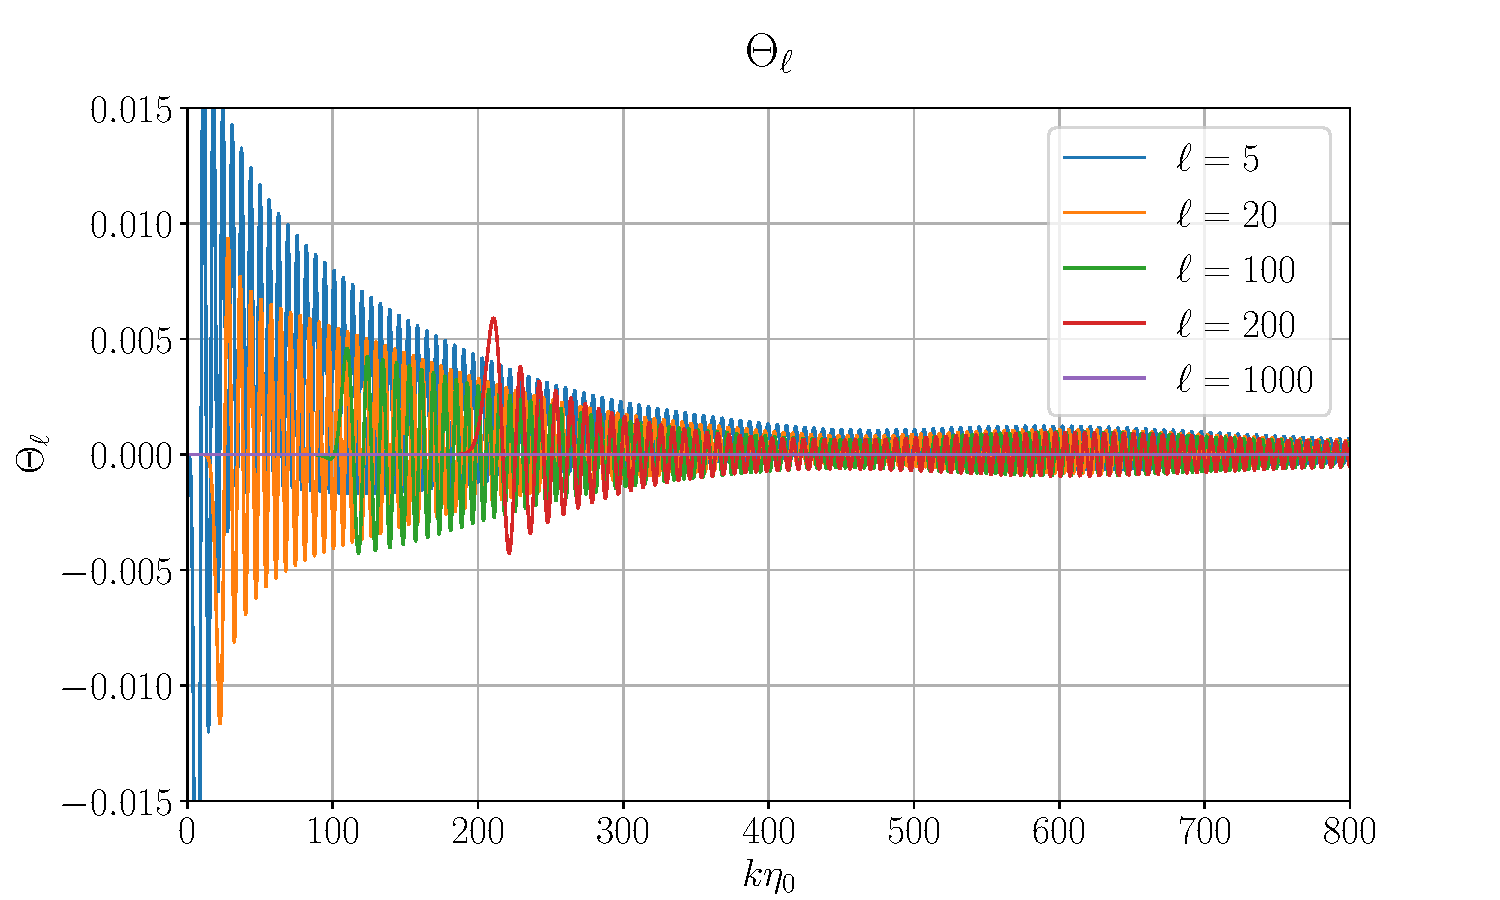
\includegraphics[width = \linewidth]{Figures/transfer.pdf}
	\caption{Transfer function $\Theta_\ell$ with $\ell\in\{5,20,100,200,1000\}$.}
	\label{fig:transfer}
\end{figure}
\begin{figure}[ht!]
	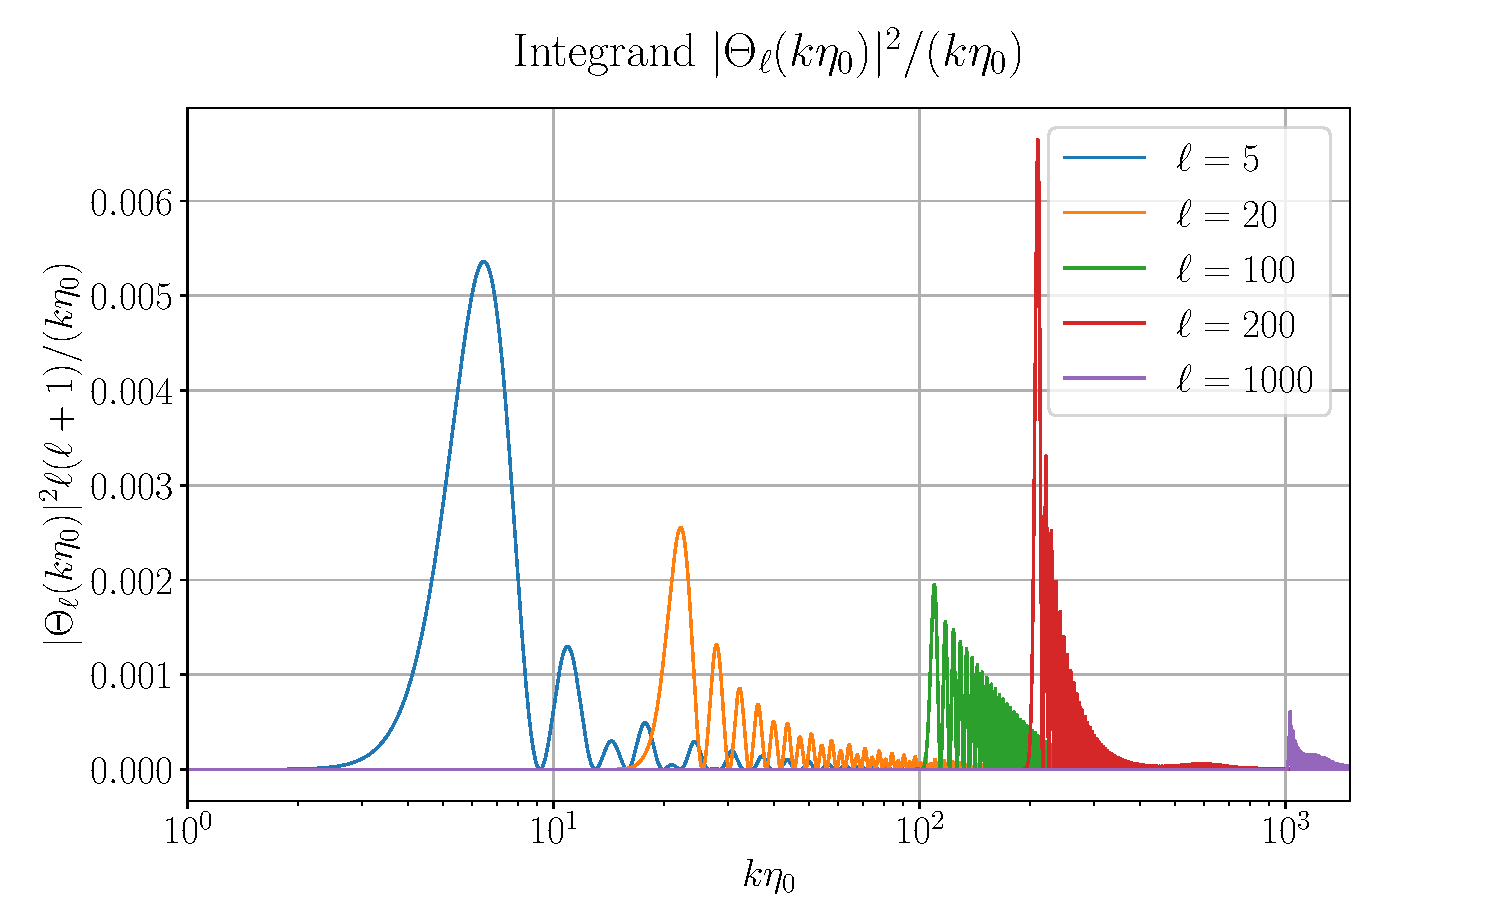
\includegraphics[width = \linewidth]{Figures/integrand.pdf}
	\caption{Integrand $|\Theta_\ell(k\eta_0)|^2$ with a normalization for each $\ell\in\{5,20,100,200,1000\}$ such that they are visible in the plot.}
	\label{fig:integrand}
\end{figure}
\subsubsection{CMB power spectrum}
We begin by looking at the CMB power spectrum which is compared to low- and high $\ell$ data from \cite{Planck:2018vyg} given in orange and red respectively depicted in Fig. \ref{fig:C_ell}. The green shaded region is the cosmic variance which was explained in the theory section. As we can see this variance is quite large for low values $\ell$ as expected from the previous discussion due to having a small number of possible data points. 
\begin{figure}[ht!]
	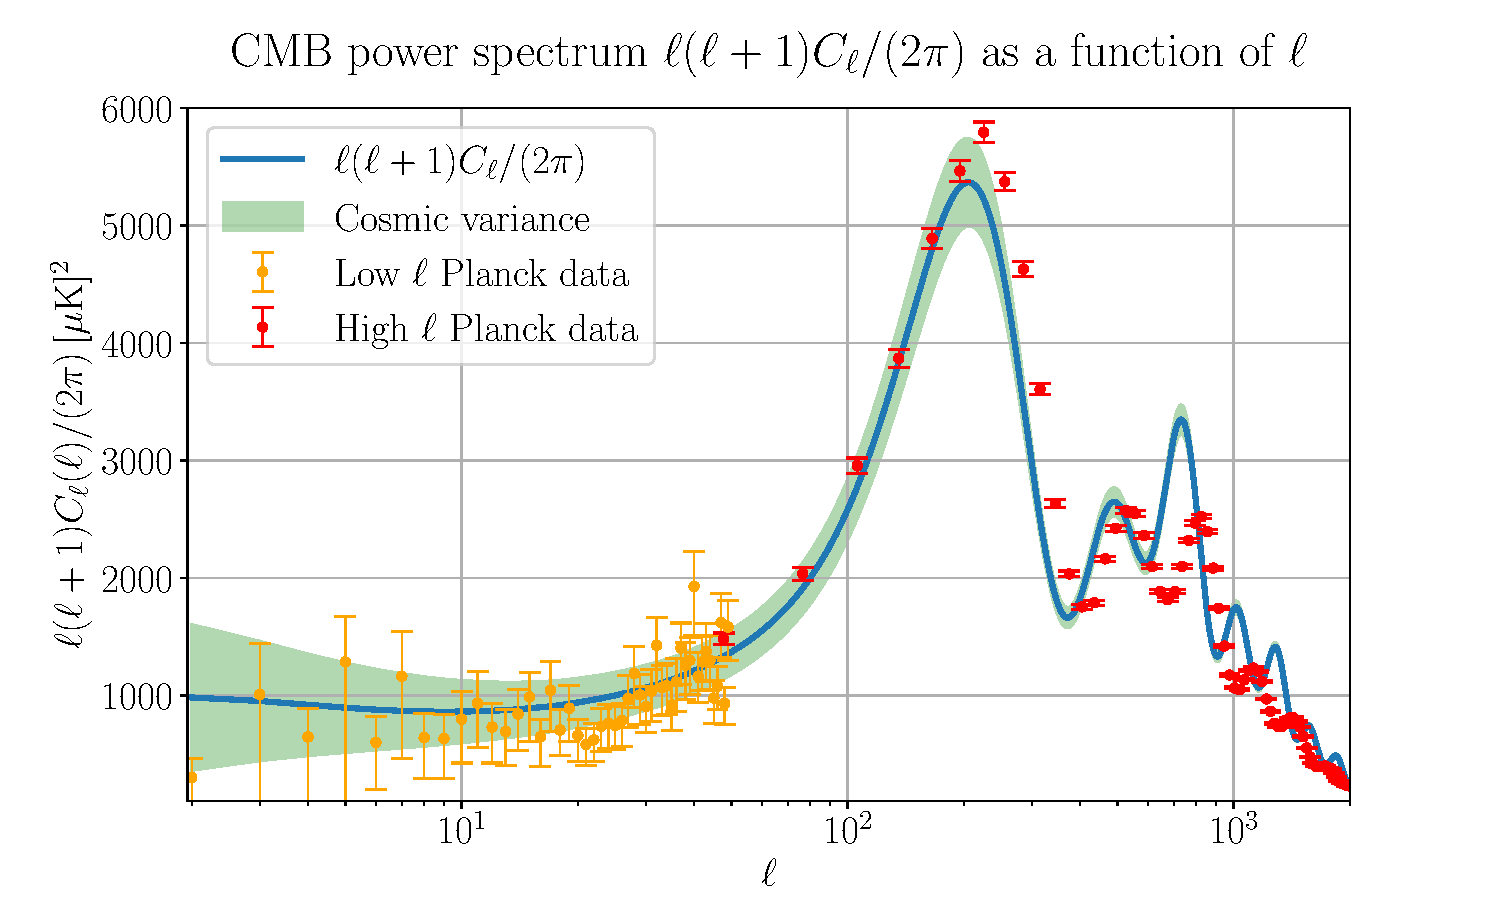
\includegraphics[width = \linewidth]{Figures/C_ell.pdf}
	\caption{CMB power spectrum $C_\ell$ plotted in conventional units and normalization as a function of photon multipole $\ell$ compared to data from \cite{Planck:2018vyg}.}
	\label{fig:C_ell}
\end{figure}

The low $\ell$ values can be seen to be relatively flat compared to the rest of the power spectra. To get a clearer the large scale physics Fig. \ref{fig:low_C_ell_vs_Planck} shows a zoomed in view of the CMB spectrum, once again compared to data from \cite{Planck:2018vyg}. Here we can see the cosmic variance in action, which forces very large error bars in this region. This is not due to ``poor'' measurements, but instead that the number of data points is simply too small for the data to be statistically accurate. We see that our numerical data is in good agreement with the experimental data, although a relatively large deviation can be seen around $20<\ell<30$. The error-bars of these data points are however still within the cosmic variance region as can be seen from the previous figure. The exact reasoning other than a potential statistical anomaly is not known, and may be a sign of new physics. The flatness of the power spectra at these scales is to be expected from the initial conditions set up by inflation. At these very large scales, as we have already seen before, there is no causal connection between the disconnected regions post inflation. Thus no changes are to be expected until one reaches scales where the modes may have entered the horizon before recombination occurred. This can be formulated mathematically via the Sachs-Wolfe effect which tells us that we expect to see a flattened curve for small $\ell$ \cite{Dodelson:2003ft}. This so-called Sachs-Wolfe plateau indicates that there should exist large scale structures in the Universe due to its high power at the smallest $\ell$'s and can be used to probe the initial conditions stemming from inflation.
\begin{figure}[ht!]
	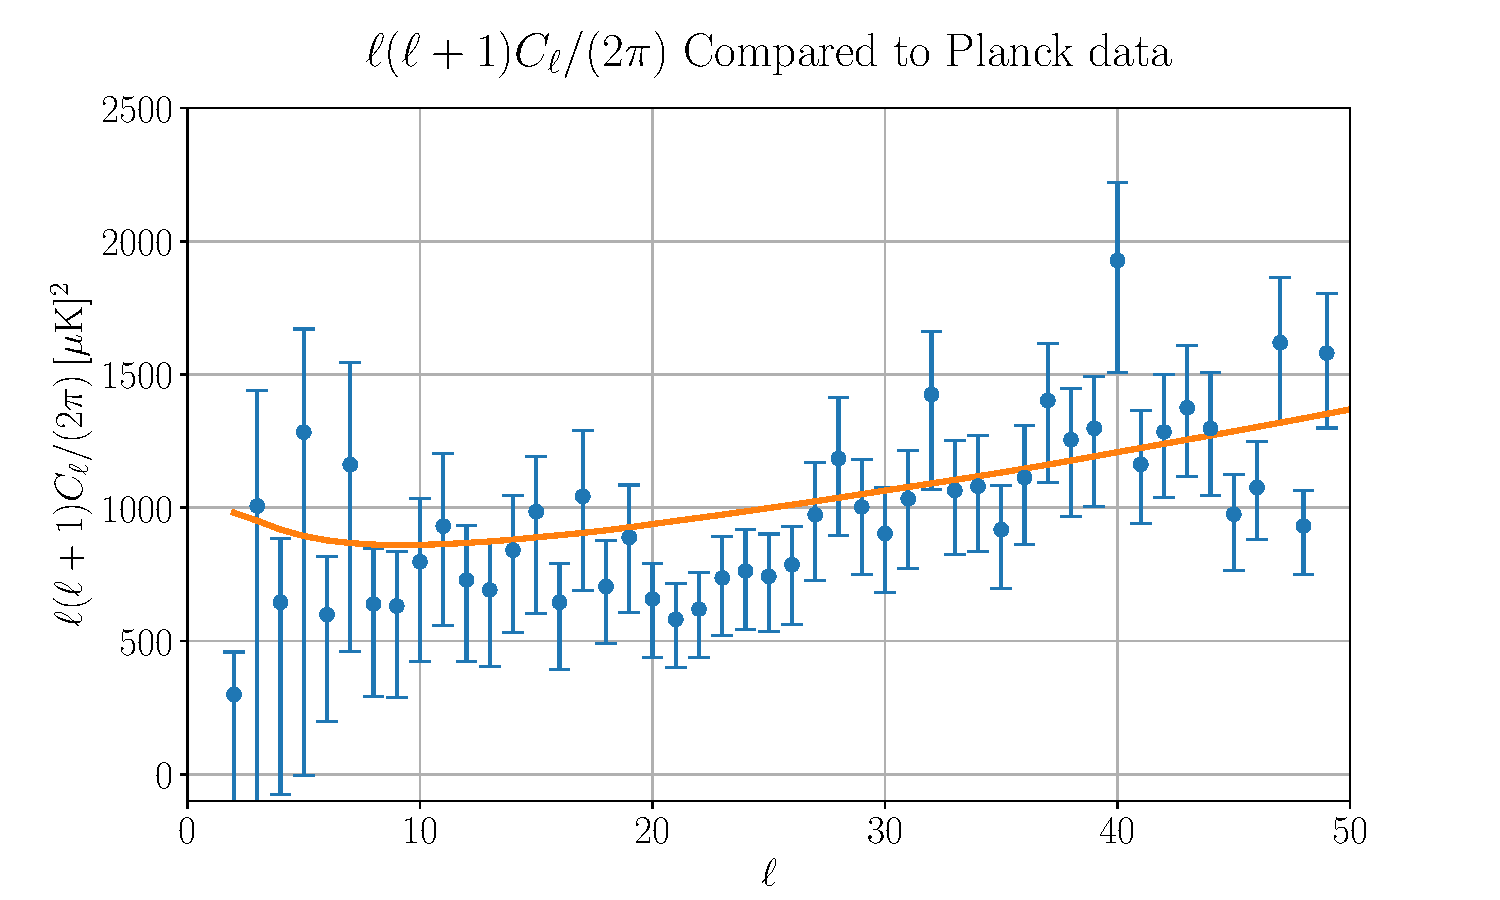
\includegraphics[width = \linewidth]{Figures/low_C_ell_vs_Planck.pdf}
	\caption{Low $\ell$ numerical values for $C_\ell$ compared to data from \cite{Planck:2018vyg}}
	\label{fig:low_C_ell_vs_Planck}
\end{figure}

Going down the scales to larger ell in Fig. \ref{fig:C_ell} we consider the first 3 peaks. These peaks are the result of the acoustic oscillations from the time before recombination. These oscillations were clearly seen in the previous section where we looked at the matter density perturbations as a function of $x$. There are some clear discrepancies in our numerical results compared to the data. This is an expected result from the fact that we have ignored any heavier elements than Hydrogen together with not accounting for effects from polarization and neutrinos. 

The first peak at $\ell\sim200$ which corresponds to the first contraction of the primordial plasma. This is the largest scale in which we see one of these compressions occur and corresponds to the scales on the order of the sound horizon at the time of last scattering. The horizontal position of this peak can be used as clear evidence to probe the inherent curvature of the Universe. If we consider that instead our universe was open but that recombination still followed the same inhomogeneities as a flat universe. In this hypothetical universe, photon paths coming towards us would converge from initially starting at larger scales but ending up having a smaller angular distance when they arrive. Thus we would perceive these photons as coming from higher $\ell$ and all the peaks in the power spectrum would shift to the right. A similar analysis can be made for a closed universe, thus the position of this peak rules out a non flat universe. Note however that there is a large degeneracy in the parameter space. For example changing the number density of baryons would also shift the peak to the right. However the peak would also grow massively in comparison to the shift.

The next two peaks are the result of a decompression and a compression respectively. Modes related to these enter the horizon and earlier times, i.e. during radiation domination. Due to this, their power are relatively low compared to the first peak due to allowing for more causal physics to have brought the plasma to an equilibrium, lowering their respective correlation at these scales. This effect essentially causes hot photons to move towards colder regions and is known as \textbf{diffusion damping}. However note that there is a so-called \textit{driving force} which causes the relative size of the third peak to grow. This can be understood by considering a coupled harmonic oscillator; Once the gravitational wells begin to flatten out in certain areas, the surplus of energy will go into increasing the amplitude of the oscillations. This is what causes the third peak to be relatively large compared to the peak before it. Our data is however not entirely in line with the observational data, and is most prominently seen for the third peak. This is due to there being an additional outward drag from the effects of neutrinos, whom we have ignored, which lowers the effect of the driving force during this second compression. Going further down we see that these peaks and troughs continue downwards in an oscillating pattern. 

The end of the spectra then corresponds to the diffusion tail, where the diffusion of hot photons quickly become more impactful due to the smaller scales. This then causes the power to quickly diminish as we go to smaller scales. Note that an important use of this data is that the ratio of the power corresponding to compression to decompression can be used as a measurement tool to determine the baryon density today. 

Further, mostly for satisfaction, we adjust our CMB power spectrum in a way which approximates the effects of polarization and neutrinos given in Fig. \ref{fig:C_ell_cheat}. Note that we do not want to interpret this figure too much as the numerical data has been altered. It is however nice to see that relatively minor alteration is needed to cheat our way to roughly account for neutrinos, heavier elements and polarization.
\begin{figure}[ht!]
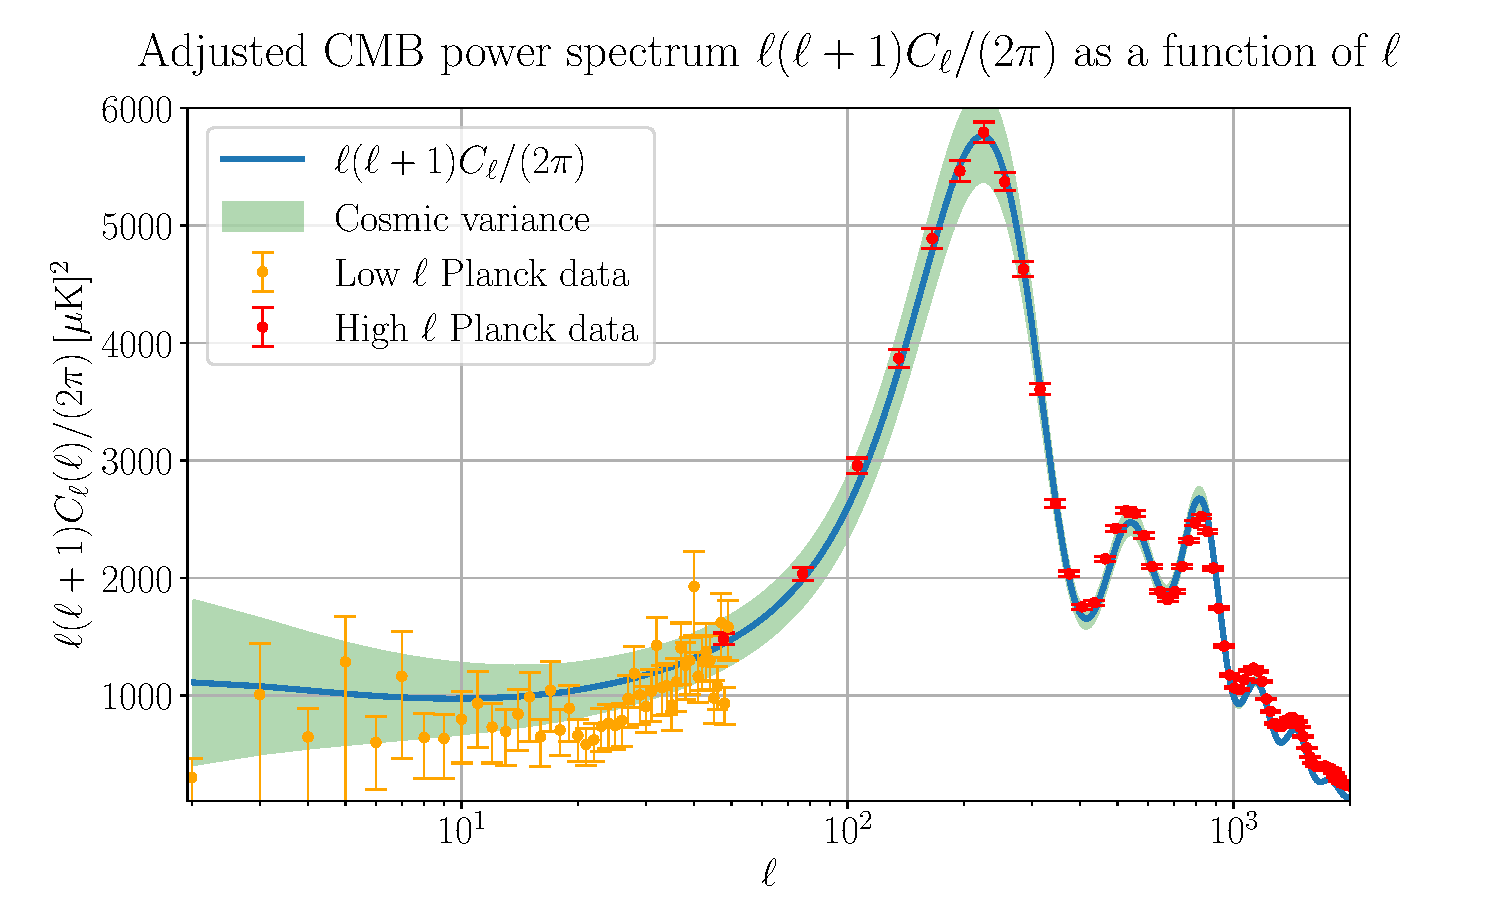
\includegraphics[width = \linewidth]{Figures/C_ell_cheat.pdf}
\caption{Adjusted CMB power spectrum where we take $\ell\to\ell^{1.018}$ and $C_\ell\to 1.13\cdot C_\ell \exp\left[-1.25\cdot10^{-5}\sqrt{2}\cdot\ell^{3/2}\right]$ compared to data from \cite{Planck:2018vyg}. Note that this is \textbf{completely arbitrary} and only done to approximate the missing shifts of peaks due to effects from helium and neutrino damping.}
\label{fig:C_ell_cheat}
\end{figure}

\subsection{Matter power spectrum}
We then have the matter power spectrum $P_\text{M}$ given in Fig. \ref{fig:Mat_pow}. Here the vertical dashed line shows the mode which enters the horizon once we have matter-radiation equality. Note that this quantity varies quite significantly as it is a function of $\Hp$ which is yet again a function of $x$ whose particular value we find via searching through a discrete array. As such, we went back to the first part of our code to increase the number of points to get a more accurate reading for this value. The matter power spectrum can be understood as an ensemble of two-point correlation functions which have then been Fourier transformed. Experimentally one would measure the distance between many galaxies and find the amplitude of how often structures seem to form given a particular distance. Then Fourier transforming these two-point correlation functions one arrives at the matter power spectrum. The left and right hand side of the $k_\text{eq}$ line can be understood as the scales which entered the horizon after and before radiation-matter equality respectively. 
\begin{figure}[ht!]
	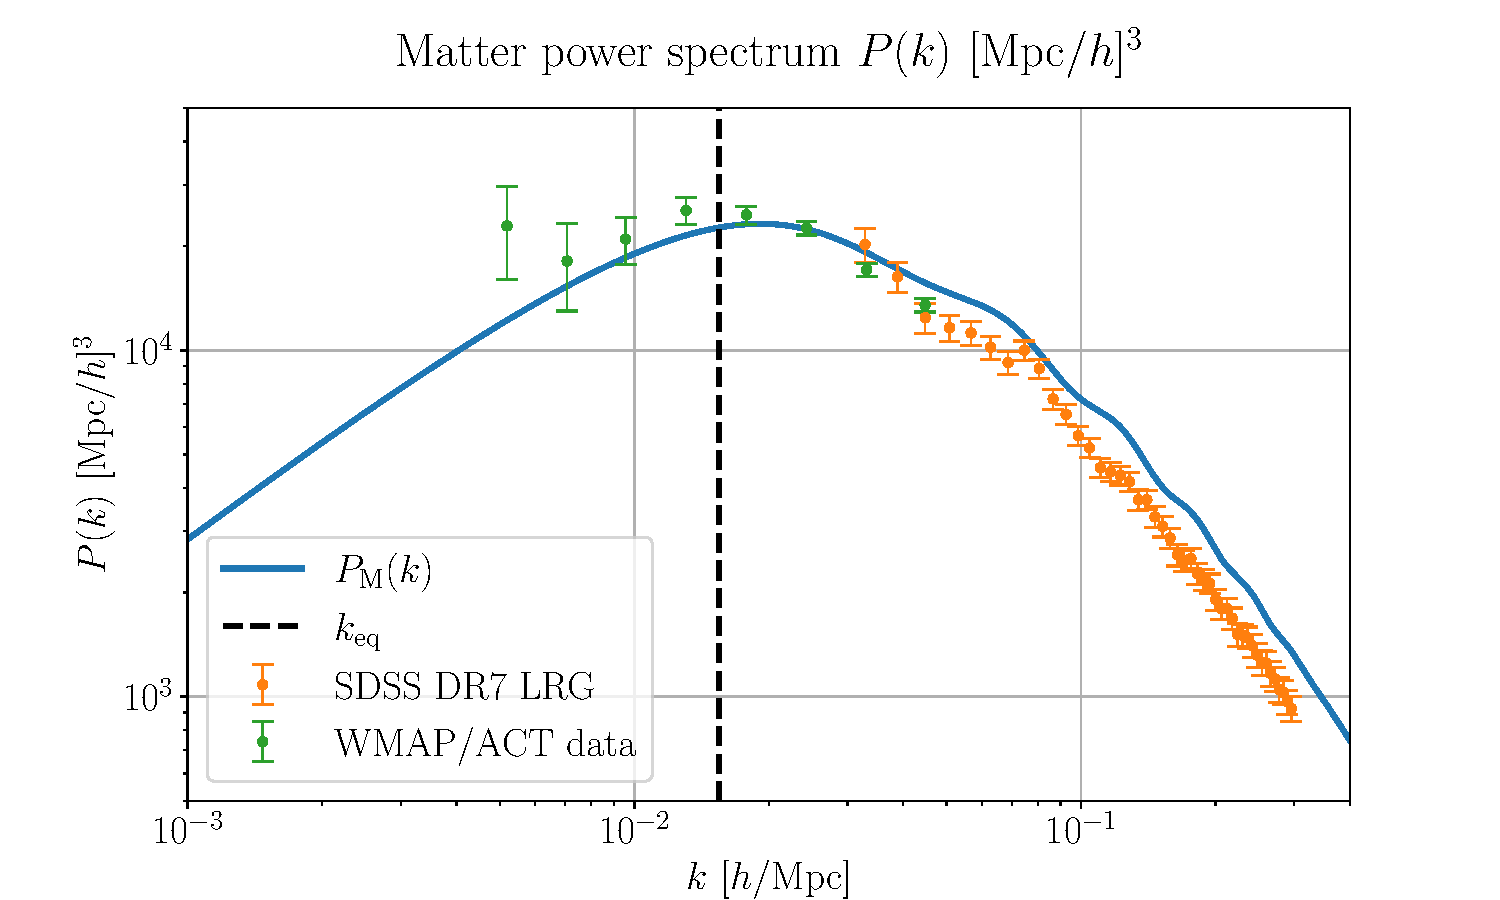
\includegraphics[width = \linewidth]{Figures/Mat_pow.pdf}
	\caption{Matter power spectrum $P_\text{M}$ as a function of Fourier mode $k$. The dotted line represents the equality scale, which is the $k$-value which corresponds to the mode entering the horizon at time of radiation-matter equality. The green points is data from \cite{Hlozek_2012} whilst the orange points are from \cite{Reid_2010}.}
	\label{fig:Mat_pow}
\end{figure}

We first consider the right hand side of $k_\text{eq}$ as this is where phenomena in the early Universe as more prominently shown. During radiation domination the baryons density fluctuations however oscillate together with the photons as we saw in the previous section in Fig. \ref{fig:b_cdm}. Since the horizon has not had much time to grow at this stage, only the smaller scales perceive some slight oscillations, which can be seen to only occur on sub-horizon scales when radiation-matter equality occurred. During this time, the CDM density perturbations grow linearly with respect to $x$ during radiation domination once their respective mode enters the horizon. Since the Universe grows at a relatively fast pace during radiation domination these overdensities are thus mostly washed out. This in turn causes the matter power spectrum to be suppressed relative to the larger scales which we can clearly see in the figure.

The left hand side is then the modes are much larger than the horizon at radiation-matter equality. These scales are too large to notice the effect of the acoustic oscillations as their modes are at super-horizon scales by the time the acoustic oscillations stop. Increasing slope that we see on the left hand side is purely due to the initial conditions which were set up by inflation. These scales have no structure formation other than the perturbations from the inflaton field. If one were to have no interactions bar the inflation perturbations matter power spectrum would simply continue to increase with $P(k)\propto k$.

The scales $k\sim k_\text{eq}$ are the ones which experience the least amount of suppression. As mentioned, these are the scales whose mode enters the horizon at the time of radiation-matter equality. At this time the expansion of the Universe is slower than during radiation domination, yet the scales are small enough to properly build up their overdensities and is thus where the matter power spectrum peaks. This overdensity peak is what is known as the \textbf{baryon acoustic oscillation peak} and corresponds to where we expect to see the largest cosmological structure form.

\subsection{Summary}
We used the data from section \ref{sec:3} together with the LOS integration technique to more efficiently be able to calculate a large ensemble of temperature fluctuations $\Theta_\ell$ using (\ref{eq:LOSx}). These were then used to calculate the CMB power spectrum $C_\ell$ with (\ref{eq:Cell_final}). Next we computed the matter power spectrum using (\ref{eq:mat_pow}) and both the power spectra were compared to data and analyzed in detail.

\end{document}